% Copyright (c) 2014  Mirantis, Inc.
%
%    Licensed under the Apache License, Version 2.0 (the "License"); you may
%    not use this file except in compliance with the License. You may obtain
%    a copy of the License at
%
%         http://www.apache.org/licenses/LICENSE-2.0
%
%    Unless required by applicable law or agreed to in writing, software
%    distributed under the License is distributed on an "AS IS" BASIS, WITHOUT
%    WARRANTIES OR CONDITIONS OF ANY KIND, either express or implied. See the
%    License for the specific language governing permissions and limitations
%    under the License.
%
\documentclass[hyperref=unicode,utf8,xcolor=pst]{beamer}
\usetheme{boxes}
\setbeamertemplate{navigation symbols}{}
%
\definecolor{mirantisred}{RGB}{211,48,26}
\setbeamercolor{titlelike}{fg=mirantisred}
\setbeamercolor{structure}{fg=mirantisred}
\hypersetup{colorlinks,urlcolor=mirantisred}
%
\usepackage[T2A]{fontenc}
%
\usepackage{graphicx}
\usepackage{fancyvrb}
\usepackage{listings}
%
\title{\fontsize{26}{0}\selectfont Ceph in Mirantis OpenStack}
\author{\vspace{-2.5mm}
\includegraphics[height=5cm]{Vector_RGB_MirantisLogo}\\Dmitry Borodaenko}
\date{Mountain View, 2014}
%
\begin{document}

\begin{frame}
	\titlepage
\end{frame}

\begin{frame}
	\frametitle{The Plan}
	\begin{enumerate}
		\item What is Ceph?
		\item What is Mirantis OpenStack?
		\item How does Ceph fit into OpenStack?
		\item What has Fuel ever done for Ceph?
		\item What does it look like?
		\item Things we've done
		\item Disk partition for Ceph OSD
		\item Cephx authentication settings
		\item Types of VM migrations
		\item Live VM migrations with Ceph
		\item Thinks we left undone
		\item Diagnostics and troubleshooting
		\item Resources
	\end{enumerate}
\end{frame}

\begin{frame}
	\frametitle{What is Ceph?}
	Ceph is a free clustered storage platform that provides unified
	object, block, and file storage.

	\begin{description}
		\item[Object Storage] RADOS objects support
			snapshotting, replication, and consistency.
		\item[Block Storage] RBD block devices are thinly
			provisioned over RADOS objects and can be
			accessed by QEMU via librbd library.\\
			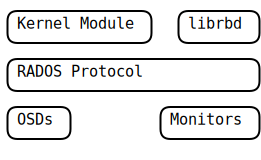
\includegraphics[height=2.5cm]{ceph-rbd}
		\item[File Storage] CephFS metadata servers (MDS)
			provide a POSIX-compliant overlay over RADOS.
	\end{description}
\end{frame}

\begin{frame}
	\frametitle{What is Mirantis OpenStack?}
	\begin{description}
		\item[OpenStack] is an open source cloud computing
			platform.\\
			\vspace{0.5ex}
			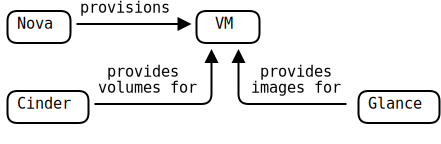
\includegraphics[height=2cm]{openstack-components}
		\item[Mirantis] ships hardened OpenStack packages and
			provides Fuel utility to simplify deployment of
			OpenStack and Ceph.
		\item[Fuel] uses Cobbler, MCollective, and Puppet to
			discover nodes, provision OS, and setup
			OpenStack services.\\
			\vspace{0.5ex}
			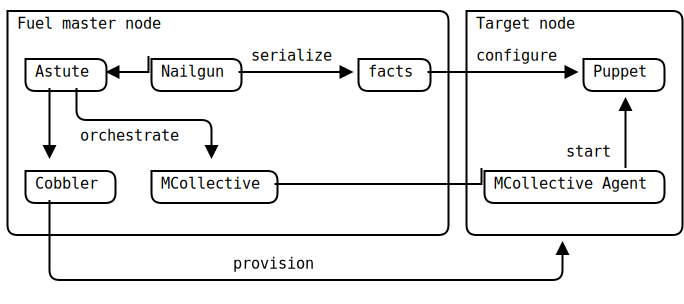
\includegraphics[height=3.8cm]{fuel-components}
	\end{description}
\end{frame}

\begin{frame}
	\frametitle{How does Ceph fit into OpenStack?}
	\begin{columns}
		\column{.6\textwidth}
		RBD drivers for OpenStack make libvirt configure the
		QEMU interface to librbd.

		\vspace{2ex}
		Ceph benefits:
		\begin{itemize}
			\item Multi-node striping and redundancy for
				block storage (Cinder volumes and Nova
				ephemeral drives)
			\item Copy-on-write cloning of images to
				volumes and instances
			\item Unified storage pool for all types of
				storage (object, block, POSIX)
			\item Live migration of Ceph-backed instances
		\end{itemize}

		\column{.3\textwidth}
		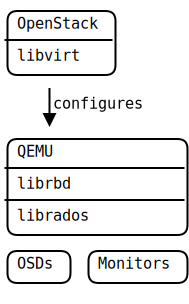
\includegraphics[height=6.5cm]{ceph-rbd-openstack}
	\end{columns}

	\vspace{2ex}
	Problems: sensitivity to clock drift, multi-site (async
	replication in Emperor), block storage density (erasure coding
	in Firefly), Swift API gap (rbd backend for Swift)
\end{frame}

\begin{frame}
	\frametitle{What has Fuel ever done for Ceph?}
	\begin{enumerate}
		\item Fuel deploys Ceph Monitors and OSDs on dedicated
			nodes or in combination with OpenStack
			components.\\
			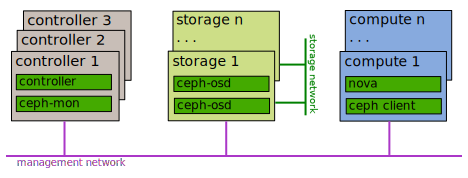
\includegraphics[height=3.7cm]{openstack-nodes}
		\item Creates partitions for OSDs when nodes are
			provisioned.
		\item Creates separate RADOS pools and sets up Cephx
			authentication for Cinder, Glance, and Nova.
		\item Configures Cinder, Glance, and Nova to use RBD
			backend with the right pools and credentials.
		\item Deploys RADOS Gateway (S3 and Swift API frontend
			to Ceph) behind HAProxy on controller nodes.
	\end{enumerate}
\end{frame}

\begin{frame}
	\frametitle{What does it look like?}
	Select storage options $\Rightarrow$ assign roles to nodes $\Rightarrow$ allocate disks:\\
	\vspace{3ex}
	\makebox[\textwidth][c]{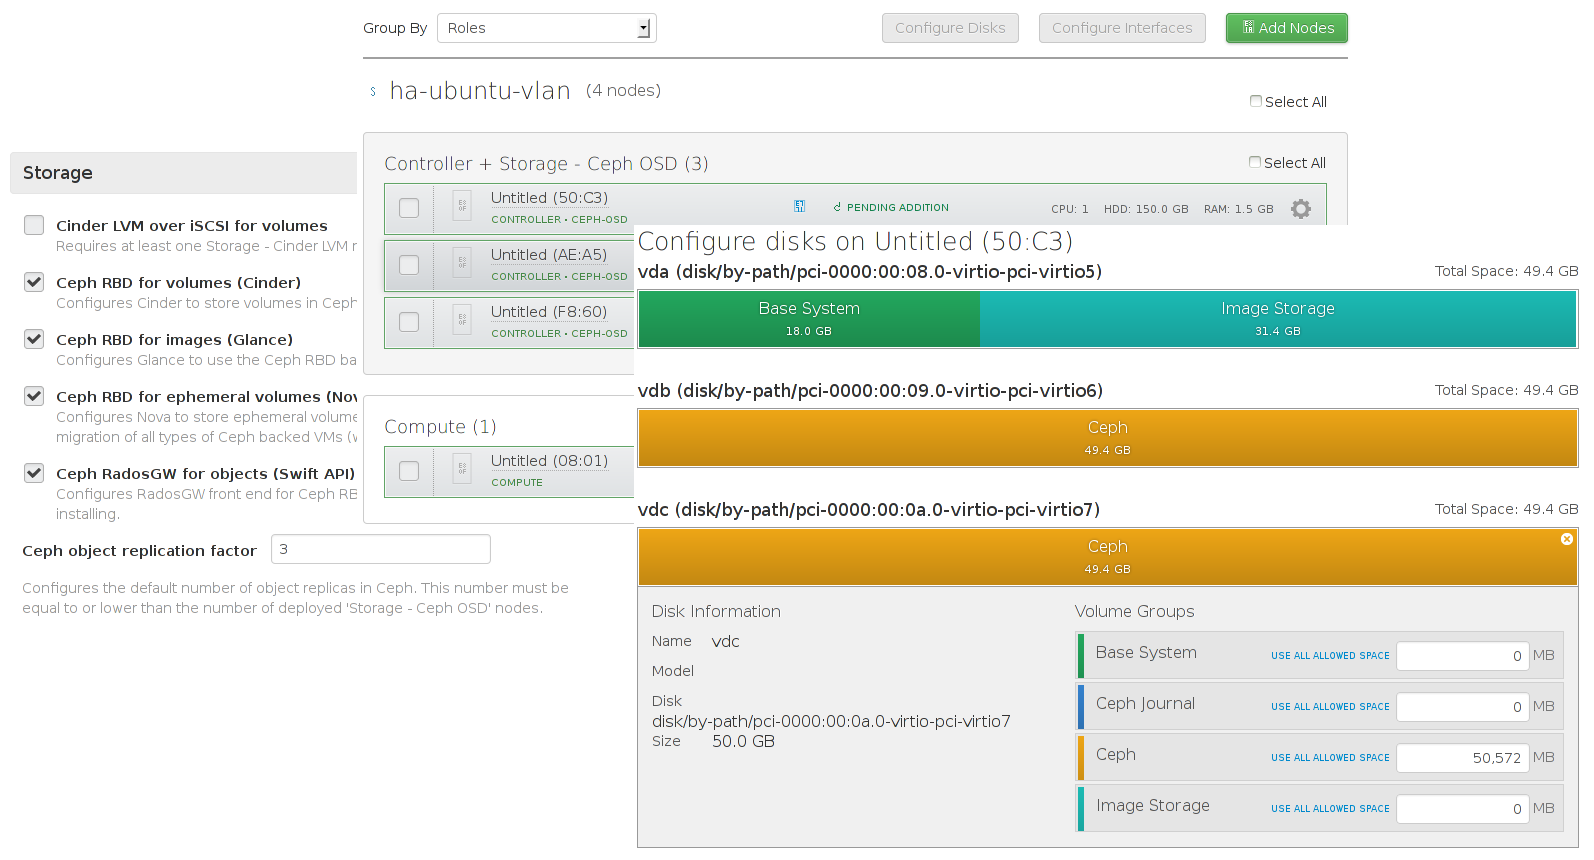
\includegraphics[width=1.18\textwidth]{fuel-ceph-screenshots}}
\end{frame}

\begin{frame}
	\frametitle{Things we've done}
	\begin{enumerate}
		\item Set the right GPT type GUIDs on OSD and journal
			partitions for udev automount rules
		\item ceph-deploy: set up root SSH between Ceph nodes
		\item Basic Ceph settings: cephx, pool size, networks
		\item Cephx: ceph auth command line can't be split
		\item Rados Gateway: has to be the Inktank's fork of
			FastCGI, set an infinite revocation interval for
			UUID auth tokens to work
		\item Patch Cinder to convert non-raw images when
			creating an RBD backed volume from Glance
		\item Patch Nova: clone RBD backed Glance images into
			RBD backed ephemeral volumes, pass RBD user to
			qemu-img
		\item Ephemeral RBD: disable SSH key injection, set up
			Nova, libvirt, and QEMU for live migrations
	\end{enumerate}
\end{frame}

\begin{frame}[fragile]
	\frametitle{Disk partitioning for Ceph OSD}
	Flow of disk partitioning information during discovery,
	configuration, provisioning, and deployment:\\
	\vspace{1ex}
	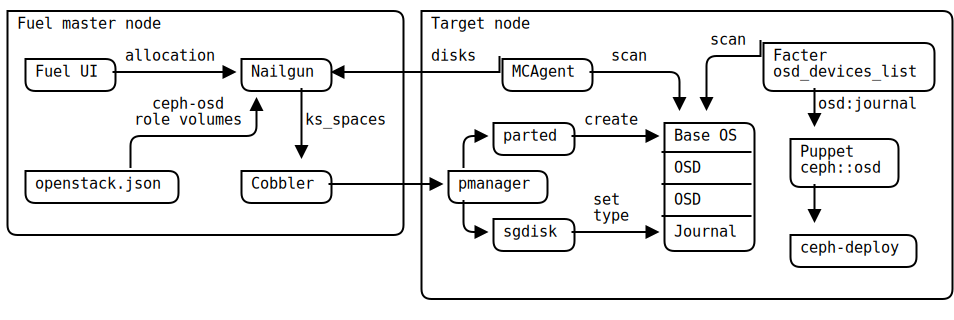
\includegraphics[height=3.7cm]{osd-disks}

	GPT partition type GUIDs according to ceph-disk:
	\lstset{language=Python,
		basicstyle=\ttfamily\footnotesize,
		keywordstyle=\color{blue}\ttfamily\footnotesize,
		stringstyle=\color{mirantisred}\ttfamily\footnotesize,
		commentstyle=\color{gray}\ttfamily\footnotesize
	}
	\begin{lstlisting}
	JOURNAL_UUID = '45b0969e-9b03-4f30-b4c6-b4b80ceff106'
	OSD_UUID     = '4fbd7e29-9d25-41b8-afd0-062c0ceff05d'
	\end{lstlisting}

	\vspace{1ex}
	If more than one device is allocated for OSD Journal, journal
	devices are evenly distributed between OSDs.
\end{frame}

\begin{frame}[fragile]
	\frametitle{Cephx authentication settings}
	\lstset{basicstyle=\ttfamily\footnotesize}

	Monitor ACL is the same for {\color{mirantisred}all} Cephx users:
	\vspace{-1ex}
	\begin{lstlisting}
	allow r
	\end{lstlisting}
	\vspace{1ex}

	OSD ACLs vary per OpenStack component:
	\vspace{-1ex}
	\begin{description}
		\item[Glance:]
			\begin{lstlisting}
			allow class-read object_prefix rbd_children,
			allow rwx pool=images
			\end{lstlisting}

		\vspace{-1.5ex}
		\item[Cinder:]
			\begin{lstlisting}
			allow class-read object_prefix rbd_children,
			allow rwx pool=volumes
			allow rx pool=images
			\end{lstlisting}

		\vspace{-1.5ex}
		\item[Nova:]
			\begin{lstlisting}
			allow class-read object_prefix rbd_children,
			allow rwx pool=volumes
			allow rx pool=images
			allow rwx pool=compute
			\end{lstlisting}
	\end{description}

	{\color{mirantisred}Watch out:} Cephx is easily tripped up by
	unexpected whitespace in ceph auth command line parameters, so
	we have to keep them all on a single line.
\end{frame}

\begin{frame}
	\frametitle{Types of VM migrations}
	{\bf OpenStack:}
	\begin{description}
		\item [Live vs offline:] Is VM stopped during migration?
		\item [Block vs shared storage vs volume-backed:] Is VM
			data shared between nodes? Is VM metadata
			(e.g. libvirt domain XML) shared?
	\end{description}

	{\bf Libvirt:}
	\begin{description}
		\item [Native vs tunneled:] Is VM state transferred
			directly between hypervisors or tunneled by
			libvirtd?
		\item [Direct vs peer-to-peer:] Is migration controlled
			by libvirt client or by source libvirtd?
		\item [Managed vs unmanaged:] Is migration controlled by
			libvirt or by hypervisor itself?
	\end{description}

	{\bf Our type:}\\
	Live, volume-backed*, native, peer-to-peer, managed.
\end{frame}

\begin{frame}
	\frametitle{Live VM migrations with Ceph}
	\begin{itemize}
		\item Enable native peer to peer live migration:\\
			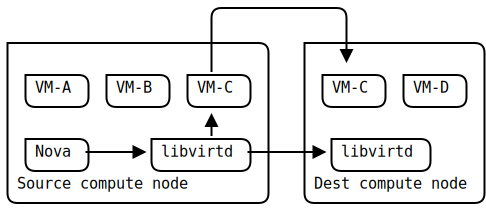
\includegraphics[height=3cm]{libvirt-p2p-migration}\\
			%libvirt flags: live, p2p, undefine-source, persist
			libvirt VIR\_MIGRATE\_* flags: LIVE, PEER2PEER,
			UNDEFINE\_SOURCE, PERSIST\_DEST
		\item Patch Nova to decouple shared volumes from shared
			libvirt metadata logic during live migration
		\item Set VNC listen address to 0.0.0.0 and block VNC
			from outside the management network in iptables
		\item Open ports 49152+ between computes for QEMU
			migrations
	\end{itemize}
\end{frame}

\begin{frame}
	\frametitle{Things we left undone}
	\begin{enumerate}
		\item Non-root user with sudo for ceph-deploy
		\item Calculate PG numbers based on the number of OSDs
		\item Ceph public network should go to a second storage
			network instead of management
		\item Dedicated Monitor nodes, list all Monitors in
			ceph.conf on each Ceph node
		\item Multi-backend configuration for Cinder
		\item A better way to configure pools for OpenStack
			services (than CEPH\_ARGS in the init script)
		\item Make Nova update VM's VNC listen address to
			vncserver\_listen of the destination compute
			after migration
		\item Replace 'qemu-img convert' with clone\_image() in
			LibvirtDriver.snapshot() in Nova
	\end{enumerate}
\end{frame}

\begin{frame}[fragile]
	\frametitle{Diagnostics and troubleshooting}
	\lstset{language=bash,basicstyle=\ttfamily\footnotesize}

	\begin{lstlisting}
	ceph -s
	ceph osd tree
	cinder create 1
	rados df
	qemu-img convert -O raw cirros.qcow2 cirros.raw
	glance image-create --name cirros-raw --is-public yes \
	  --container-format bare --disk-format raw < cirros.raw
	nova boot --flavor 1 --image cirros-raw vm0
	nova live-migration vm0 node-3
	\end{lstlisting}

	\begin{description}
		\item[disk partitioning failed during provisioning] --
			check if traces of previous partition tables are
			left on any drives
		\item['ceph-deploy config pull' failed] -- check if the
			node can ssh to the primary controller over
			management network
		\item[HEALTH\_WARN: clock skew detected] -- check your
			ntpd settings, make sure your NTP server is
			reachable from all nodes
		\item[ENOSPC when storing small objects in RGW] -- try
			setting a smaller rgw object stripe size
	\end{description}
\end{frame}

\begin{frame}
	\frametitle{Resources}
	Read the docs:\\
	\url{http://ceph.com/docs/next/rbd/rbd-openstack/}\\
	\url{http://docs.mirantis.com/fuel/fuel-4.0/}\\
	\url{http://libvirt.org/migration.html}\\
	\url{http://docs.openstack.org/admin-guide-cloud/content/ch\_introduction-to-openstack-compute.html}

	\vspace{2ex}
	Get the code:\\
	\begin{itemize}
		\item \href{http://software.mirantis.com/}{Mirantis OpenStack} ISO image and VirtualBox scripts,\\
		\item \href{https://github.com/stackforge/fuel-library/tree/master/deployment/puppet/ceph}{ceph} Puppet module for Fuel,\\
		\item Josh Durgin's \href{https://github.com/jdurgin/nova/commits/havana-ephemeral-rbd}{havana-ephemeral-rbd} branch for Nova.
	\end{itemize}

	\vspace{2ex}
	Vote on Nova bugs:\\
	\href{https://bugs.launchpad.net/fuel/+bug/1226351}{\#1226351},
	\href{https://bugs.launchpad.net/fuel/+bug/1261675}{\#1261675},
	\href{https://bugs.launchpad.net/fuel/+bug/1262450}{\#1262450},
	\href{https://bugs.launchpad.net/fuel/+bug/1262914}{\#1262914}.

	\vspace{2ex}
	Sign up for
	\href{http://bit.ly/JZIgRD}{Mirantis and Inktank webcast on Ceph
	and OpenStack}.
\end{frame}

\end{document}
